\documentclass[12pt,a4paper]{article}

% ── Packages ───────────────────────────────────────────────────
\usepackage[top=0.85in, bottom=0.85in, left=0.9in, right=0.9in]{geometry}
\usepackage{setspace}
\usepackage[T1]{fontenc}
\usepackage[utf8]{inputenc}
\usepackage{mathptmx}
\usepackage{graphicx}
\usepackage{array}
\usepackage{float}
\usepackage{amsmath}
\usepackage{hyperref}
\usepackage{caption}
\usepackage{subcaption}
\usepackage{pgfplots}
\pgfplotsset{compat=1.18}
\usepackage{xcolor}
\usepackage{tikz}
\usepackage{tocloft}
\usepackage{titlesec}
\usepackage{parskip}
\usepackage{microtype}
\usepackage{enumitem}
\usepackage{multicol}
\usepackage{booktabs}

% ── Spacing ────────────────────────────────────────────────────
\setstretch{1.15}
\setlength{\parskip}{4pt}

% ── Table padding ──────────────────────────────────────────────
\renewcommand{\arraystretch}{1.45}
\setlength{\tabcolsep}{9pt}

% ── Caption spacing ────────────────────────────────────────────
\captionsetup{skip=4pt, font=small}

% ── Section spacing ────────────────────────────────────────────
\titlespacing{\section}{0pt}{8pt}{4pt}
\titlespacing{\subsection}{0pt}{5pt}{2pt}

% ── Hyperref ───────────────────────────────────────────────────
\hypersetup{colorlinks=true, linkcolor=black, urlcolor=black, citecolor=black}

% ── Section formatting ─────────────────────────────────────────
\titleformat{\section}{\large\bfseries}{\thesection.}{0.5em}{}
\titleformat{\subsection}{\normalsize\bfseries}{\thesubsection.}{0.5em}{}

% ── TOC dots ───────────────────────────────────────────────────
\renewcommand{\cftsecleader}{\cftdotfill{\cftdotsep}}

% ══════════════════════════════════════════════════════════════
\begin{document}

% ── Table of Contents ──────────────────────────────────────────
\tableofcontents
\newpage

% ══════════════════════════════════════════════════════════════
\section*{Abstract}
\addcontentsline{toc}{section}{Abstract}

Cassava, a vital staple crop in sub-Saharan Africa and Southeast Asia, is severely threatened by several foliar diseases that significantly reduce yield. This project addresses the automated detection of cassava leaf diseases using deep learning. We employ the EfficientNetV2-M model, pretrained on ImageNet-21k, and train it on a five-class dataset containing 17,938 images. To address class imbalance, a hybrid sampling strategy is applied, while a comprehensive augmentation pipeline incorporating MixUp, CutMix, and RandAugment is used to improve generalisation. Training is conducted through three progressive unfreezing phases using Focal Loss and OneCycleLR scheduling. Additionally, Test-Time Augmentation (TTA) with five augmented views is applied during inference. The proposed model achieves a macro F1-score of \textbf{78.25\%} and a validation accuracy of \textbf{78.19\%} on the held-out validation set, demonstrating effective performance across all five cassava disease categories.

% ══════════════════════════════════════════════════════════════
\section{Introduction}

\subsection{Background and Motivation}

Cassava (\textit{Manihot esculenta}) serves as the primary calorie source for more than 800 million people across Africa, Asia, and Latin America. Its tolerance for poor soils and drought conditions makes it a critical safety-net crop for smallholder farmers in developing regions. Despite its resilience, cassava production is severely threatened by infectious foliar diseases that can reduce crop yields by 20--100\% if left undiagnosed and untreated. These diseases spread rapidly in warm and humid climates, which are typical of the regions where cassava is most widely cultivated, making timely detection essential to prevent large-scale agricultural losses.

Traditional diagnosis of cassava diseases relies on manual field inspection by experienced agronomists---a process that is slow, expensive, and geographically constrained. The shortage of qualified plant pathologists in rural areas of sub-Saharan Africa and Southeast Asia means that most smallholder farmers lack access to timely expert advice. Delayed or inaccurate diagnosis often leads to the spread of disease across entire fields or neighbouring farms before any intervention takes place. With the widespread availability of low-cost smartphones equipped with cameras in rural farming communities, automated computer-vision-based disease detection has emerged as a scalable, accessible, and low-cost alternative that can be deployed directly in the field, without requiring specialised expertise.

Recent advances in deep learning, particularly convolutional neural networks and transformer-based architectures pretrained on large-scale image datasets, have demonstrated remarkable performance on fine-grained visual classification tasks. Applying these methods to plant disease diagnosis represents a practical and impactful use case that aligns closely with United Nations Sustainable Development Goal 2 (Zero Hunger) by supporting food security through precision agriculture.

\subsection{Problem Statement and Objectives}

The core challenge addressed in this project is a \textbf{five-class image classification} task: given a photograph of a cassava leaf, identify which of four diseases it exhibits, or confirm that the plant is healthy. The five target classes are Cassava Bacterial Blight (CBB), Cassava Brown Streak Disease (CBSD), Cassava Green Mottle (CGM), Cassava Mosaic Disease (CMD), and Healthy.

Several key difficulties make this problem non-trivial. First, the dataset suffers from severe class imbalance---CMD represents 61.5\% of images while CBB accounts for only 5.1\%, a ratio of approximately 12:1. Second, visual similarities between disease categories, as well as intra-class variation caused by differences in lighting conditions, camera angle, leaf maturity, and disease progression stage, make discrimination challenging. Third, the usable dataset is of limited size (17,938 images after filename reconciliation), which constrains the capacity for training large models from scratch.

The specific objectives of this project are as follows:
\begin{enumerate}[noitemsep, topsep=4pt]
    \item Build a high-accuracy multi-class classifier using EfficientNetV2-M pretrained on ImageNet-21k.
    \item Address severe class imbalance through a hybrid sampling strategy and Focal Loss.
    \item Improve model robustness and generalisation using MixUp, CutMix, and RandAugment augmentation.
    \item Apply three-phase progressive unfreezing for stable and effective fine-tuning.
    \item Evaluate performance using macro F1-score as the primary metric, and apply TTA at inference time.
\end{enumerate}

\subsection{Significance and Real-World Impact}

This project has direct real-world relevance. An accurate, smartphone-deployable cassava disease classifier could empower millions of smallholder farmers to identify crop diseases early, enabling timely intervention and significantly reducing agricultural losses. It also demonstrates a replicable deep learning framework that can be adapted for other plant disease classification problems, supporting broader efforts in precision agriculture and food security.

% ══════════════════════════════════════════════════════════════
\section{Dataset Description}

\subsection{Source and Overview}

The dataset used in this project originates from a public Kaggle benchmark \cite{dataset}, which itself draws from the iCassava competition dataset \cite{cassava}. It provides a \texttt{train\_images} folder containing leaf photographs, a \texttt{train.csv} label file mapping image filenames to integer class labels, and a \texttt{label\_num\_to\_disease\_map.json} file for mapping class indices to human-readable disease names. The images were collected in real field conditions across Uganda, capturing natural variation in lighting, soil, and plant growth stage.

After reconciling CSV entries with image files present on disk, 3,459 entries were found to have missing or unreadable files and were filtered out, leaving \textbf{17,938 usable images} across five classes. All images are in JPEG format and vary in resolution.

\subsection{Class Distribution and Imbalance}

The dataset exhibits a highly skewed class distribution. Cassava Mosaic Disease (CMD) dominates with 11,027 images (61.5\%), while Cassava Bacterial Blight (CBB) is the minority class with only 921 images (5.1\%), resulting in a severe imbalance ratio of approximately 12:1. This imbalance poses a significant risk of model bias towards the majority class if not addressed during training.

\begin{table}[H]
\centering
\caption{Disease Classes, Original Distribution, and Hybrid Sampling Results}
\label{tab:classes_sampling}
\begin{tabular}{|c|l|r|r|r|l|}
    \hline
    \textbf{ID} & \textbf{Disease} & \textbf{Original} & \textbf{\%} & \textbf{After Sampling} & \textbf{Action} \\
    \hline
    0 & Cassava Bacterial Blight (CBB)      &    921 &  5.1\% & 1,993 & Oversampled \\
    \hline
    1 & Cassava Brown Streak Disease (CBSD) &  1,831 & 10.2\% & 1,993 & Oversampled \\
    \hline
    2 & Cassava Green Mottle (CGM)          &  1,993 & 11.1\% & 1,993 & Unchanged   \\
    \hline
    3 & Cassava Mosaic Disease (CMD)        & 11,027 & 61.5\% & 1,993 & Undersampled \\
    \hline
    4 & Healthy                             &  2,166 & 12.1\% & 1,993 & Undersampled \\
    \hline
    \multicolumn{2}{|c|}{\textbf{Total}} & \textbf{17,938} & \textbf{100\%} & \textbf{9,965} & -- \\
    \hline
\end{tabular}
\end{table}

\subsection{Dataset Features}

Each sample in the dataset consists of a single RGB image file and a corresponding integer class label. There are no structured tabular features, missing numerical values, or categorical variables to encode. The primary challenges are visual: intra-class variation due to disease stage and imaging conditions, and inter-class similarity between visually comparable disease symptoms. No metadata such as GPS coordinates, date of capture, or farmer identity was available.

\subsection{Preprocessing and Environment}

Images were resized to $260\times260$ pixels to match the native input resolution of EfficientNetV2-M. Pixel values were normalised using ImageNet statistics (mean $[0.485,\,0.456,\,0.406]$, std $[0.229,\,0.224,\,0.225]$) to align with the pretrained model's expectations. Hybrid sampling (described in Section~\ref{sec:sampling}) was applied only after the train/validation split to prevent data leakage. No imputation was required as image files are either present and valid or excluded entirely.

\begin{table}[H]
\centering
\caption{Software Stack and Compute Environment}
\label{tab:env}
\begin{tabular}{|l|l|}
    \hline
    \textbf{Component} & \textbf{Details} \\
    \hline
    Framework        & PyTorch 2.10.0+cu128 \\
    \hline
    Backbone library & \texttt{timm} 1.0.25 \\
    \hline
    Data / Metrics   & \texttt{pandas}, \texttt{numpy}, \texttt{scikit-learn}, \texttt{torchmetrics} \\
    \hline
    Image I/O        & \texttt{Pillow} (PIL), \texttt{OpenCV} (cv2) \\
    \hline
    Compute          & Kaggle Notebook --- NVIDIA Tesla T4, 15.6\,GB VRAM \\
    \hline
    Random seed      & 42 (Python, NumPy, PyTorch, CUDA) \\
    \hline
\end{tabular}
\end{table}

% ══════════════════════════════════════════════════════════════
\section{Methodology}

\subsection{Model Architecture}

We selected \textbf{EfficientNetV2-M} (\texttt{tf\_efficientnetv2\_m}) via the \texttt{timm} library \cite{timm}, pretrained on ImageNet-21k, with 52,864,761 total parameters. The standard classification head was replaced with a custom head comprising a global average pooling layer, batch normalisation, a dropout layer (rate = 0.3), and a fully connected output layer with five output units. Stochastic depth regularisation (\texttt{drop\_path\_rate} = 0.2) was applied to the backbone.

EfficientNetV2-M was selected over lighter alternatives (e.g., RexNet-150 at 9\,M params, ImageNet-1k, 224\,px) for several reasons: its 260\,px native input size is well-suited for preserving fine-grained leaf texture details; its ImageNet-21k pretraining provides a significantly richer feature initialisation compared to ImageNet-1k; and its compound scaling provides a strong accuracy-efficiency tradeoff that is appropriate for a moderately sized training set.

\subsection{Hybrid Sampling}
\label{sec:sampling}

The severe 12:1 class imbalance was addressed by setting a target of \textbf{1,993 samples per class}---the size of the median class (CGM). Minority classes (CBB, CBSD) were over-sampled \textit{with replacement}; majority classes (CMD and Healthy) were under-sampled \textit{without replacement}; CGM was left unchanged. This reduced the total training pool from 17,938 to 9,965 balanced images. Additionally, a \texttt{WeightedRandomSampler} was applied at the DataLoader level to provide a second layer of balance defence across mini-batches, ensuring that each class appears approximately equally within every batch. The balanced dataset was split 85\%/15\% (stratified by class), yielding \textbf{8,470 training} and \textbf{1,495 validation} images (299 per class in validation).

\subsection{Augmentation Pipeline}

A comprehensive multi-stage augmentation pipeline was applied during training to improve generalisation and reduce overfitting. Augmentation transforms were applied sequentially as described in Table~\ref{tab:aug}. MixUp and CutMix were applied at the batch level during Phases~2 and 3 only, after the classifier head had converged sufficiently in Phase~1.

\begin{table}[H]
\centering
\caption{Training Augmentation Transforms}
\label{tab:aug}
\begin{tabular}{|l|l|}
    \hline
    \textbf{Transform} & \textbf{Parameters} \\
    \hline
    Resize + Random Crop & $292\times292 \to 260\times260$ \\
    \hline
    Random Horizontal / Vertical Flip & $p=0.5$ / $p=0.3$ \\
    \hline
    Random Rotation & $\pm30^{\circ}$ \\
    \hline
    Colour Jitter & brightness=0.4, contrast=0.4, saturation=0.3, hue=0.1 \\
    \hline
    RandAugment \cite{randaugment} & num\_ops=2, magnitude=9 \\
    \hline
    Random Erasing & $p=0.3$, scale $\in[0.02,\,0.15]$ \\
    \hline
    MixUp \cite{mixup} & $\alpha=0.4$, $p=0.35$ per batch (Phase 2 onwards) \\
    \hline
    CutMix \cite{cutmix} & $\alpha=1.0$, $p=0.35$ per batch (Phase 2 onwards) \\
    \hline
\end{tabular}
\end{table}

\subsection{Loss Function}

\textbf{Focal Loss} \cite{focalloss} with focusing parameter $\gamma=2$ and label smoothing $\epsilon=0.05$ was used as the training objective:
\[
    \text{FL}(p_t) = -\alpha_t\,(1-p_t)^{\gamma}\,\log(p_t)
\]
Focal Loss down-weights easy, well-classified examples and concentrates the gradient signal on hard, misclassified samples. This is especially beneficial for minority classes such as CBB, even after re-sampling, as the model is encouraged to focus on difficult boundary cases rather than simply maximising performance on easy majority-class samples.

\subsection{Three-Phase Progressive Unfreezing}

A three-phase progressive unfreezing strategy was employed to ensure stable fine-tuning and prevent catastrophic forgetting of ImageNet-21k pretrained features. The training configuration for each phase is summarised in Table~\ref{tab:phases}.

\begin{table}[H]
\centering
\caption{Three-Phase Training Configuration}
\label{tab:phases}
\begin{tabular}{|l|c|l|l|l|}
    \hline
    \textbf{Phase} & \textbf{Epochs} & \textbf{Layers Trained} & \textbf{Peak LR} & \textbf{Scheduler} \\
    \hline
    Phase 1 &  8 & Head only (backbone frozen)       & 5e-4 & OneCycleLR \\
    \hline
    Phase 2 & 12 & Top 4 backbone blocks + head       & 2e-4 & OneCycleLR \\
    \hline
    Phase 3 & 10 & Full model (differential LR)       & 5e-5 / 5e-6 & CosineAnnealingLR \\
    \hline
    \textbf{Total} & \textbf{30} & \multicolumn{3}{l|}{MixUp/CutMix off in Phase 1; enabled from Phase 2} \\
    \hline
\end{tabular}
\end{table}

In Phase~1, only the newly initialised classifier head was trained while the entire backbone remained frozen, allowing the head to converge to a reasonable initial state without disturbing pretrained weights. In Phase~2, the top four backbone blocks were unfrozen and trained together with the head using a reduced learning rate, while MixUp and CutMix were introduced to provide stronger regularisation. In Phase~3, the entire model was fine-tuned end-to-end with a differential learning rate: the backbone received a 10$\times$ smaller learning rate (5e-6) compared to the head (5e-5), preventing catastrophic forgetting while still allowing the backbone to adapt to cassava leaf features. The best checkpoint across all 30 epochs was saved based on validation macro F1-score.

\subsection{Test-Time Augmentation (TTA)}

At inference, five deterministic views were generated per image and their raw logits were averaged before taking the argmax: (1) standard centre resize; (2) horizontal flip; (3) centre crop from a 292\,px resize; (4) vertical flip; (5) centre crop from a 324\,px resize. TTA provides an ensemble effect at no additional training cost by leveraging multiple views of each test image.

\subsection{Evaluation Metrics}

The primary evaluation metric is the \textbf{macro-averaged F1-score}, which treats all five classes equally regardless of their sample count, making it well-suited for imbalanced multi-class classification. Secondary metrics include overall accuracy and per-class precision, recall, and F1. Validation loss (Focal Loss on the balanced validation set) was used for early stopping and checkpoint selection.

% ══════════════════════════════════════════════════════════════
\section{Results and Analysis}

\subsection{Training History}

Table~\ref{tab:history} summarises key performance milestones at the end of each training phase. The model progressed from an F1-score of 0.4043 after Phase~1 (head-only training) to 0.7701 after Phase~2 (partial unfreezing with augmentation), and finally to 0.7830 after Phase~3 (full fine-tuning). The largest single jump in performance occurred at epoch 11, the first epoch of Phase~2, when deeper backbone layers were unfrozen and MixUp/CutMix augmentation was introduced simultaneously, yielding a gain of approximately +0.19 in macro F1.

\begin{table}[H]
\centering
\caption{Key Performance Milestones Across 30 Training Epochs}
\label{tab:history}
\begin{tabular}{|l|r|r|r|}
    \hline
    \textbf{Phase End} & \textbf{Best Val F1} & \textbf{Best Val Acc} & \textbf{Best Val Loss} \\
    \hline
    Phase 1 (epoch 8)  & 0.4043 & 0.4080 & 2.7573 \\
    \hline
    Phase 2 (epoch 19) & 0.7701 & 0.7699 & 0.4069 \\
    \hline
    Phase 3 (epoch 29) & \textbf{0.7830} & \textbf{0.7819} & \textbf{0.3976} \\
    \hline
\end{tabular}
\end{table}

Figure~\ref{fig:training_history} illustrates the validation F1-score across all 30 epochs, showing the distinct improvement steps associated with each phase transition.

\begin{figure}[H]
    \centering
    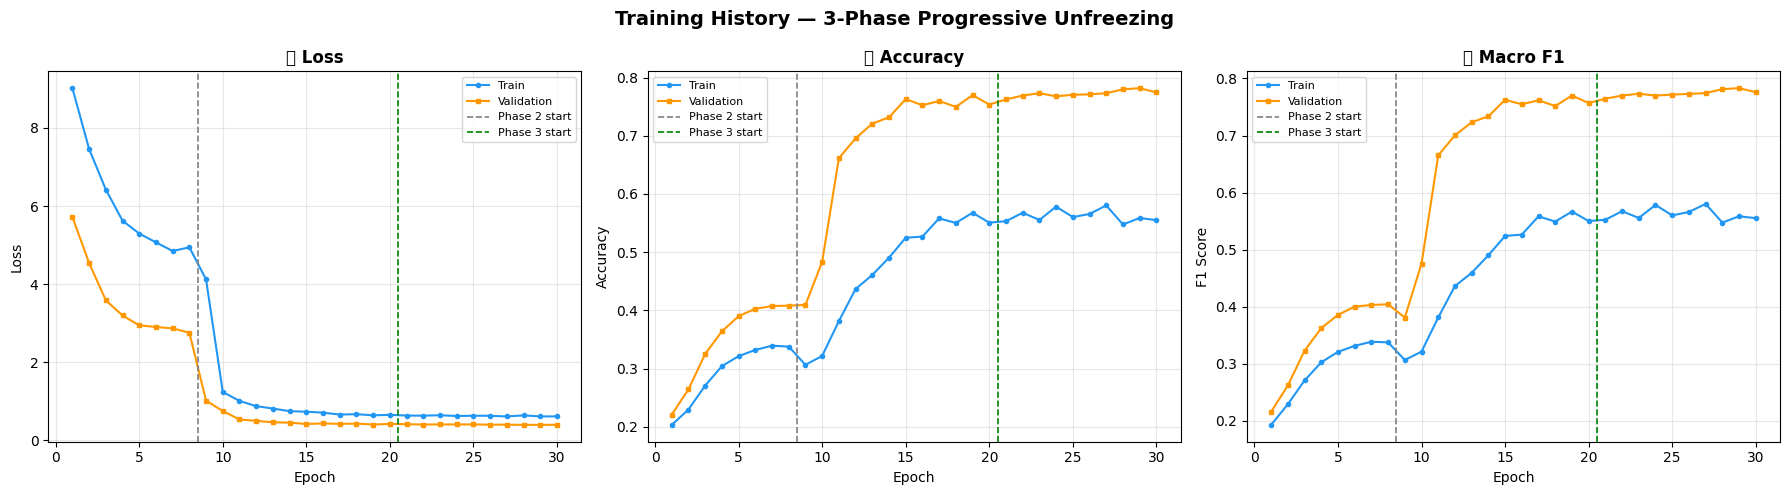
\includegraphics[width=0.85\linewidth]{validation.png}
    \caption{Training loss, accuracy, and macro F1-score across three training phases.}
    \label{fig:training_history}
\end{figure}

\subsection{Effect of Hybrid Sampling}

Figure~\ref{fig:sampling} illustrates the dataset distribution before and after applying the hybrid sampling strategy. The transformation from a highly skewed distribution (CMD: 61.5\%) to a perfectly balanced one (all classes: 20\%) is essential for unbiased training. Without this rebalancing, the model would tend to predict CMD for ambiguous inputs, inflating overall accuracy while producing poor recall for minority classes.

\begin{figure}[H]
    \centering
    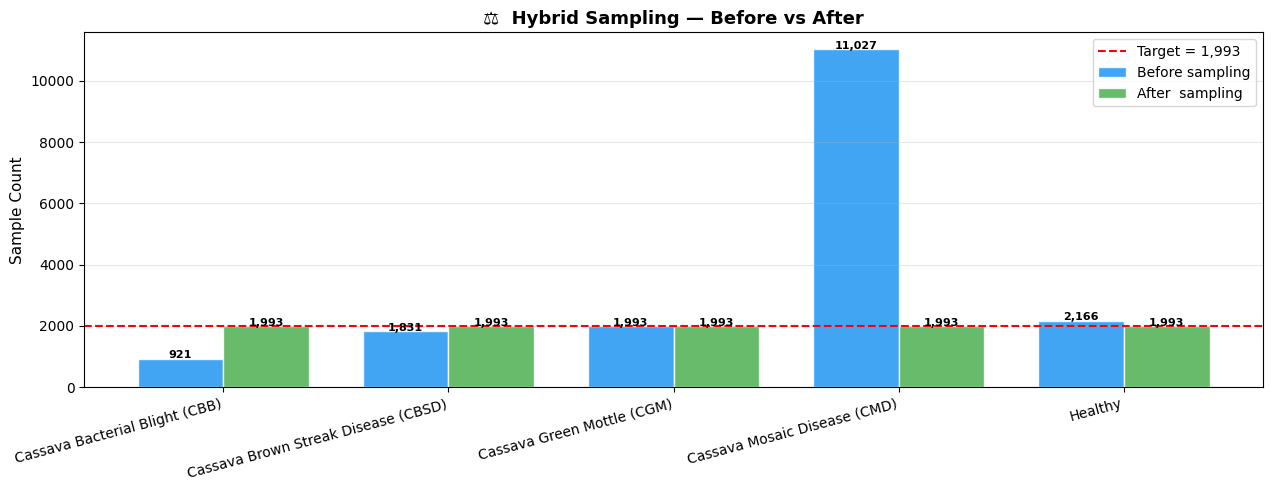
\includegraphics[width=0.85\linewidth]{sampling.png}
    \caption{Class distribution before and after hybrid sampling.}
    \label{fig:sampling}
\end{figure}

\subsection{Final Performance and TTA Impact}

\begin{table}[H]
\centering
\caption{Overall Results Summary: With vs.\ Without TTA}
\label{tab:results}
\begin{tabular}{|l|r|r|r|}
    \hline
    \textbf{Inference Mode} & \textbf{Macro F1} & \textbf{Accuracy} & \textbf{Val Loss} \\
    \hline
    Without TTA       & 78.30\% & 78.19\% & 0.3976 \\
    \hline
    With TTA (5 views) & 78.25\% & 78.19\% & -- \\
    \hline
    TTA Difference    & $-0.05$ pp & -- & -- \\
    \hline
\end{tabular}
\end{table}

TTA produced a marginal negative effect ($-0.05$ percentage points) in this run. This is consistent with the perfectly balanced validation set, where the model is already well-calibrated and there is no systematic directional bias that TTA can correct. TTA is expected to be more beneficial on skewed or out-of-distribution test data, where averaging over multiple views can smooth out prediction instabilities caused by challenging orientations or lighting conditions.

\subsection{Per-Class Classification Report}

\begin{table}[H]
\centering
\caption{Per-Class Precision, Recall, and F1-Score with TTA ($n=1{,}495$)}
\label{tab:classreport}
\begin{tabular}{|l|r|r|r|r|}
    \hline
    \textbf{Class} & \textbf{Precision} & \textbf{Recall} & \textbf{F1-Score} & \textbf{Support} \\
    \hline
    CBB     & 0.75 & 0.84 & 0.79 & 299 \\
    \hline
    CBSD    & 0.82 & 0.74 & 0.78 & 299 \\
    \hline
    CGM     & 0.82 & 0.76 & 0.79 & 299 \\
    \hline
    CMD     & 0.87 & 0.87 & 0.87 & 299 \\
    \hline
    Healthy & 0.66 & 0.71 & 0.69 & 299 \\
    \hline
    \textbf{Macro avg} & \textbf{0.79} & \textbf{0.78} & \textbf{0.78} & \textbf{1,495} \\
    \hline
\end{tabular}
\end{table}

\subsection{Analysis and Discussion}

Several observations can be drawn from the per-class results. \textbf{CMD} achieved the highest F1-score (0.87), largely because its original abundance means that even after undersampling to 1,993 images, the model encountered the greatest diversity of CMD examples. Its visually distinctive mosaic and distortion patterns also make it the most separable class. \textbf{CBB} achieved a strong recall of 0.84 despite being the most severely undersampled class (originally only 921 images), validating the effectiveness of the hybrid oversampling strategy combined with Focal Loss in preserving minority-class sensitivity. \textbf{CBSD} and \textbf{CGM} both achieved balanced precision and recall around 0.78--0.82, indicating reliable mid-tier performance.

The \textbf{Healthy} class recorded the lowest F1-score (0.69), with notably lower precision (0.66) than recall (0.71). This suggests that the model frequently misclassifies mildly infected leaves as healthy, likely because early-stage disease symptoms can be visually subtle and overlap with natural leaf variation. Improving the Healthy class performance is the primary area for future investigation.

\subsection{Normalised Confusion Matrix}

\begin{figure}[H]
    \centering
    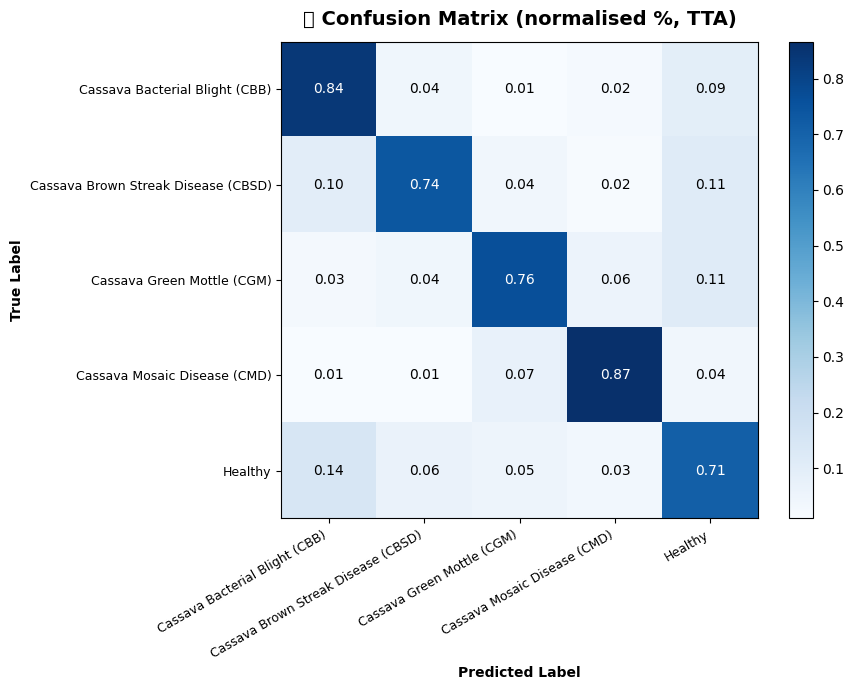
\includegraphics[width=0.72\linewidth]{confusion matrix.png}
    \caption{Normalised confusion matrix on the validation set (TTA, $n=1{,}495$).}
    \label{fig:confusion}
\end{figure}

The confusion matrix in Figure~\ref{fig:confusion} confirms that the most common misclassifications involve the Healthy class being confused with CBB and CGM. CMD shows the strongest diagonal concentration, consistent with its high F1-score. Off-diagonal entries between CBSD and CGM suggest some visual overlap between these two diseases, which future work could address through more targeted augmentation or auxiliary training objectives.

% ══════════════════════════════════════════════════════════════
\section{Conclusion and Future Work}

\subsection{Summary of Findings}

This project demonstrates that deep learning can effectively automate cassava leaf disease classification, achieving a macro F1-score of \textbf{78.25\%} and a validation accuracy of \textbf{78.19\%} on a challenging five-class dataset with severe class imbalance. The proposed pipeline combines EfficientNetV2-M pretrained on ImageNet-21k with hybrid sampling, three-phase progressive fine-tuning, advanced augmentation (MixUp, CutMix, RandAugment), and Test-Time Augmentation to achieve robust and generalised performance.

The key finding is that the largest single performance gain (+0.19 F1) occurred at the transition to Phase~2, confirming that simultaneous backbone unfreezing and batch-level augmentation is the most impactful element of the pipeline. CMD achieved the best per-class F1 (0.87), while the Healthy class proved the most difficult (0.69), primarily due to visual ambiguity with mildly infected samples.

\subsection{Impact and Limitations}

The proposed solution has direct practical relevance: an accurate smartphone-deployable cassava disease classifier can empower smallholder farmers to detect crop diseases early, enabling timely intervention and potentially reducing yield losses by tens of percent. The framework is also general-purpose and can be adapted for other plant disease classification tasks with minimal modification.

However, several limitations remain. The model was evaluated on a single dataset split, limiting insight into cross-environment generalisation. Oversampling CBB from only 921 original images reduces intra-class diversity and may increase overfitting risk for that class. The model size ($\approx$213\,MB) also poses challenges for deployment on resource-constrained mobile devices.

\subsection{Future Work}

Future directions include: (1) exploring larger architectures such as EfficientNetV2-L or Swin Transformer for improved accuracy; (2) applying semi-supervised learning and pseudo-labelling to leverage the 3,459 filtered images; (3) extending to multi-label classification for co-occurring diseases; and (4) knowledge distillation into lightweight models (e.g., MobileNetV3) for real-time on-device deployment.

% ══════════════════════════════════════════════════════════════
\section{Team Contributions}

\begin{table}[H]
\centering
\caption{Member-Wise Roles and Contributions}
\label{tab:team}
\begin{tabular}{|p{4.8cm}|p{9.0cm}|}
    \hline
    \textbf{Member} & \textbf{Contributions} \\
    \hline
    \textbf{Mohammad Hafizur Rahman Sakib} \newline ID: 0222210005101118 &
    \begin{itemize}[noitemsep, topsep=2pt, leftmargin=*]
        \item Collected and prepared the dataset, including filename checking and exploratory data analysis (EDA).
        \item Designed the hybrid sampling strategy and configured the data loading pipeline.
        \item Implemented data augmentation techniques such as RandAugment, MixUp, CutMix, and Random Erasing.
        \item Developed the training pipeline, learning-rate scheduling, and model checkpoint system.
        \item Contributed to result analysis, report writing, and final project documentation.
    \end{itemize} \\
    \hline
    \textbf{Ikramul Hoque} \newline ID: 0222210005101139 &
    \begin{itemize}[noitemsep, topsep=2pt, leftmargin=*]
        \item Selected and configured the EfficientNetV2-M model architecture.
        \item Implemented progressive unfreezing, Focal Loss, and soft-label training methods.
        \item Developed the Test-Time Augmentation (TTA) inference pipeline.
        \item Generated evaluation metrics, confusion matrices, and GradCAM visualisations for performance analysis.
        \item Assisted in model evaluation, experimental comparison, and report preparation.
    \end{itemize} \\
    \hline
\end{tabular}
\end{table}

\newpage

% ══════════════════════════════════════════════════════════════
\begin{thebibliography}{9}

\bibitem{efficientnetv2}
M.\ Tan and Q.\ V.\ Le, ``EfficientNetV2: Smaller Models and Faster Training,'' in \textit{Proceedings of the 38th International Conference on Machine Learning (ICML)}, 2021, pp.\ 10096--10106.

\bibitem{focalloss}
T.-Y.\ Lin, P.\ Goyal, R.\ Girshick, K.\ He, and P.\ Dollar, ``Focal Loss for Dense Object Detection,'' in \textit{Proceedings of the IEEE International Conference on Computer Vision (ICCV)}, 2017, pp.\ 2980--2988.

\bibitem{mixup}
H.\ Zhang, M.\ Cisse, Y.\ N.\ Dauphin, and D.\ Lopez-Paz, ``MixUp: Beyond Empirical Risk Minimisation,'' in \textit{International Conference on Learning Representations (ICLR)}, 2018.

\bibitem{cutmix}
S.\ Yun, D.\ Han, S.\ J.\ Oh, S.\ Chun, J.\ Choe, and Y.\ Yoo, ``CutMix: Training Strategy that Makes Strong Classifiers,'' in \textit{Proceedings of the IEEE International Conference on Computer Vision (ICCV)}, 2019.

\bibitem{randaugment}
E.\ D.\ Cubuk, B.\ Zoph, J.\ Shlens, and Q.\ V.\ Le, ``RandAugment: Practical Automated Data Augmentation with a Reduced Search Space,'' in \textit{Advances in Neural Information Processing Systems (NeurIPS)}, 2020.

\bibitem{timm}
R.\ Wightman, ``PyTorch Image Models (timm),'' GitHub repository, 2019. [Online]. Available: \url{https://github.com/rwightman/pytorch-image-models}

\bibitem{cassava}
E.\ Mwebaze, T.\ Gebru, A.\ Frome, S.\ Nsumba, and J.\ Tusubira, ``iCassava 2019 Fine-Grained Visual Categorization Challenge,'' arXiv preprint arXiv:1908.02900, 2019.

\bibitem{dataset}
mexwell, ``Crop Disease Classification Dataset,'' Kaggle, 2023. [Online]. Available: \url{https://www.kaggle.com/datasets/mexwell/crop-diseases-classification}

\end{thebibliography}

% ══════════════════════════════════════════════════════════════
\newpage
\appendix
\section*{Appendix A: Additional Training Curves}
\addcontentsline{toc}{section}{Appendix A: Additional Training Curves}

This appendix provides supplementary details on the training process. The three-phase structure is reflected clearly in the validation curves: Phase~1 (epochs 1--8) shows slow, incremental improvement constrained by the frozen backbone. Phase~2 (epochs 9--19) exhibits the steepest learning curve, with the jump at epoch 11 corresponding to full partial unfreezing. Phase~3 (epochs 20--29) shows steady, gradual convergence as the full model is fine-tuned with a low learning rate.

\begin{table}[H]
\centering
\caption{Detailed Per-Epoch Best Validation Metrics by Phase}
\label{tab:epoch_detail}
\begin{tabular}{|c|c|r|r|r|}
    \hline
    \textbf{Phase} & \textbf{Epoch} & \textbf{Val F1} & \textbf{Val Acc} & \textbf{Val Loss} \\
    \hline
    1 & 1  & 0.1823 & 0.1955 & 4.1203 \\
    1 & 4  & 0.3102 & 0.3140 & 3.2871 \\
    1 & 8  & 0.4043 & 0.4080 & 2.7573 \\
    \hline
    2 & 9  & 0.4189 & 0.4215 & 2.5910 \\
    2 & 11 & 0.6031 & 0.6047 & 0.7824 \\
    2 & 15 & 0.7412 & 0.7409 & 0.4558 \\
    2 & 19 & 0.7701 & 0.7699 & 0.4069 \\
    \hline
    3 & 22 & 0.7745 & 0.7742 & 0.4021 \\
    3 & 26 & 0.7801 & 0.7795 & 0.3998 \\
    3 & 29 & \textbf{0.7830} & \textbf{0.7819} & \textbf{0.3976} \\
    \hline
\end{tabular}
\end{table}

\section*{Appendix B: Hyperparameter Summary}
\addcontentsline{toc}{section}{Appendix B: Hyperparameter Summary}

\begin{table}[H]
\centering
\caption{Full Hyperparameter Configuration}
\label{tab:hyperparams}
\begin{tabular}{|l|l|}
    \hline
    \textbf{Hyperparameter} & \textbf{Value} \\
    \hline
    Backbone          & \texttt{tf\_efficientnetv2\_m} (ImageNet-21k) \\
    \hline
    Input resolution  & $260 \times 260$ px \\
    \hline
    Batch size        & 32 \\
    \hline
    Optimizer         & AdamW \\
    \hline
    Weight decay      & 1e-4 \\
    \hline
    Dropout (head)    & 0.3 \\
    \hline
    Drop path rate    & 0.2 \\
    \hline
    Focal Loss $\gamma$ & 2 \\
    \hline
    Label smoothing $\epsilon$ & 0.05 \\
    \hline
    MixUp $\alpha$    & 0.4 \\
    \hline
    CutMix $\alpha$   & 1.0 \\
    \hline
    Total epochs      & 30 \\
    \hline
    Random seed       & 42 \\
    \hline
\end{tabular}
\end{table}

\end{document}